\section{Anforderungen an die Software}

\subsection{Kriterienvergleich der Barrierefreiheit zwischen Web- und Desktopanwendungen}
\label{subsec: Kriterienvergleich der Barrierefreiheit zwischen Web- und Desktopanwendungen}

Die Normen der \ac{WCAG} 2.0 bzw. der \ac{WCAG} 2.1 sind an erster Stelle entweder an Inhalten von Webseiten oder Inhalten der webbasierten Anwendungen orientiert. Allerdings kommen diese Normen auch im Bereich Mobile-Anwendungen zum Einsatz.\footnote{The World Wide Web Consortium (W3C) \cite{w3c}}

Auf der anderen Seite haben die Normen der \ac{BITV} die Regel neben Webseiten und Mobilen-Anwendungen auf jeder grafischen Programmoberfläche verallgemeinert, die einer der folgenden Bedingungen betrifft:\footnote{Die Barrierefreie-Informationstechnik-Verordnung 2.0 \cite{BITV}}

\begin{itemize}
	\item Die Software ist für Angebote, Anwendungen oder Dienste, die Verwaltungsabläufe elektronisch unterstützen, einschließlich der Verfahren zur elektronischen Vorgangsbearbeitung 
	und elektronischen Aktenführung, gedacht.
	\item Die Software wird zur Nutzung an öffentlichen Stellen bereitgestellt.
\end{itemize}

Somit stehen offiziell für Desktopanwendungen, die nicht an öffentlichen Stellen genutzt werden und die nicht für die Nutzung von allen Menschen gedacht sind, noch keine feste Regeln für digitale Barrierefreiheit. Das betrifft Unternehmenssoftware, welche nur intern im Unternehmen genutzt wird. Aus diesem Grund wird ein Vergleich zwischen Web- und Desktopanwendungen gezogen, um herauszufinden, wie viel die Umsetzung der digitalen Barrierefreiheit in Desktopanwendungen von Webseiten bzw. webbasierten Anwendungen abweicht.

Für diesen Zweck werden die wesentlichen Eigenschaften der Web- und Desktopanwendungen betrachtet und es wird bewertet, ob die Eigenschaften einen Einfluss auf die Umsetzung der digitalen Barrierefreiheit in den Desktopanwendungen haben.

In der \cref{tab:Webanwendungen vs Desktopanwendung}\footnote{Eigene Darstellung} sind die Unterschiede wichtiger Eigenschaften\footnote{Cyber-Solutions \cite{CyberSolutions}} zwischen Web- und Desktopanwendungen betrachtet und es wird bewertet, ob die Eigenschaften die Umsetzung der digitalen Barrierefreiheit in den Desktopanwendungen verhindern können.

\begin{table}[H]
	\caption{Wesentliche Unterschiede zwischen  Web- und Desktopanwendungen}
	\label{tab:Webanwendungen vs Desktopanwendung}
	\centering
	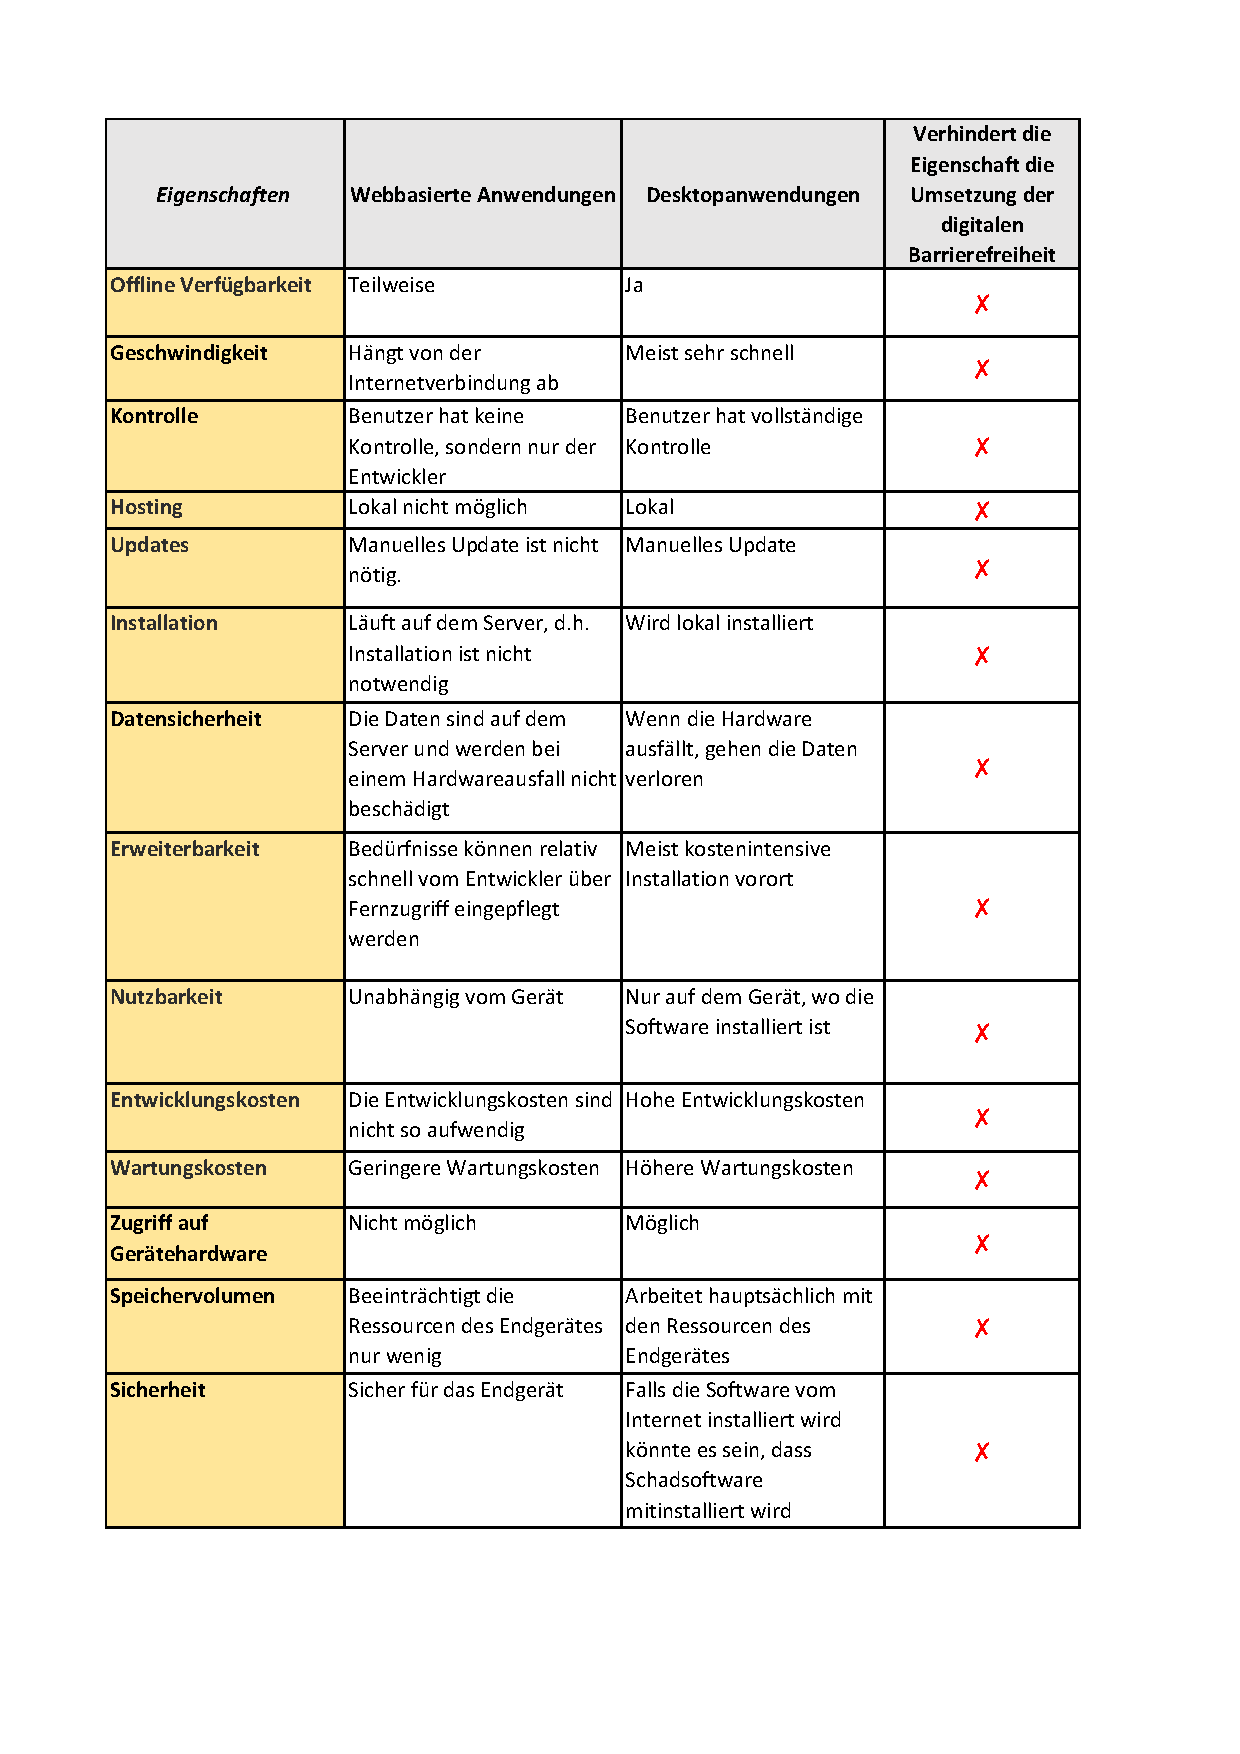
\includegraphics[width=6in]{Webanwendungen vs Desktopanwendung.pdf}
\end{table}

Anhand der Auswertung der Eigenschaften in \cref{tab:Webanwendungen vs Desktopanwendung} werden die Normen der \ac{WCAG} 2.0 bzw. der \ac{WCAG} 2.1 für Desktopanwendungen genauso behandelt, wie für webbasierte Anwendungen. Es werden keine bestimmten Ausnahmen für die Desktopanwendungen gemacht, es sei denn, die Umsetzung einer bestimmten Richtlinie bzw. eines bestimmten Erfolgskriteriums ist ausschließlich für Webseiten gedacht und in den Desktopanwendungen nicht möglich.

\subsubsection{Umsetzbare Kriterien in den aktuellen Desktopanwendungen}
\label{subsec: Umsetzbare Kriterien}

Es wird nun die Umsetzbarkeit aller Richtlinien der \ac{WCAG} 2.0 bzw. der \ac{WCAG} 2.1 in Dialogen der Desktopanwendungen des Unternehmens untersucht. Demzufolge können einige  Erfolgskriterien ausgeschlossen werden. Eine Richtlinie gilt erst als umsetzbar in Dialogen der Desktopanwendungen des Unternehmens, wenn alle Erfolgskriterien der Konformitätsstufe A erfüllt werden können. Außerdem wird jede Entscheidung, ob eine Richtlinie bzw. ein Erfolgskriterium erfüllt werden kann, begründet. In \cref{subsec: Soll-Zustand der Desktopanwendungen} werden dementsprechend die in den Desktopanwendungen umsetzbare Richtlinien präsentiert und es werden Beispiele für Techniken zur Beseitigung der digitalen Barrieren bezüglich der Erfolgskriterien vorgeschlagen, um die betroffenen Richtlinien erfüllen zu können.

In der folgenden Tabelle werden alle Richtlinien und jedes ihrer Erfolgskriterien mit der entsprechenden Konformitätsstufe präsentiert und auf die Umsetzbarkeit in Dialogen der Desktopanwendungen hin geprüft. Für den Zweck haben zwei Sitzungen mit Fachexperten der StyleGuide-Gruppe Gruppe\change{Ein paar Wörter über die Gruppe} sowie der Dokumentationsabteilung des Unternehmens stattgefunden. In den Sitzungen wurde untersucht, ob die Erfolgskriterien in Dialogen der aktuellen Software und für die neue Software des Unternehmens umsetzbar, nicht umsetzbar oder nicht relevant für Dialoge der Desktopanwendungen sind. Des Weiteren wurde entschieden, dass Erfolgskriterien der Konformitätsstufe AAA nicht umgesetzt werden. Aus diesem Grund werden diese nicht betrachtet.

\unsure{Reicht dann dieser Absatz aus?}

\addcontentsline{lot}{table}{2 \hspace{1.5em} Bewertung der Richtlinien}
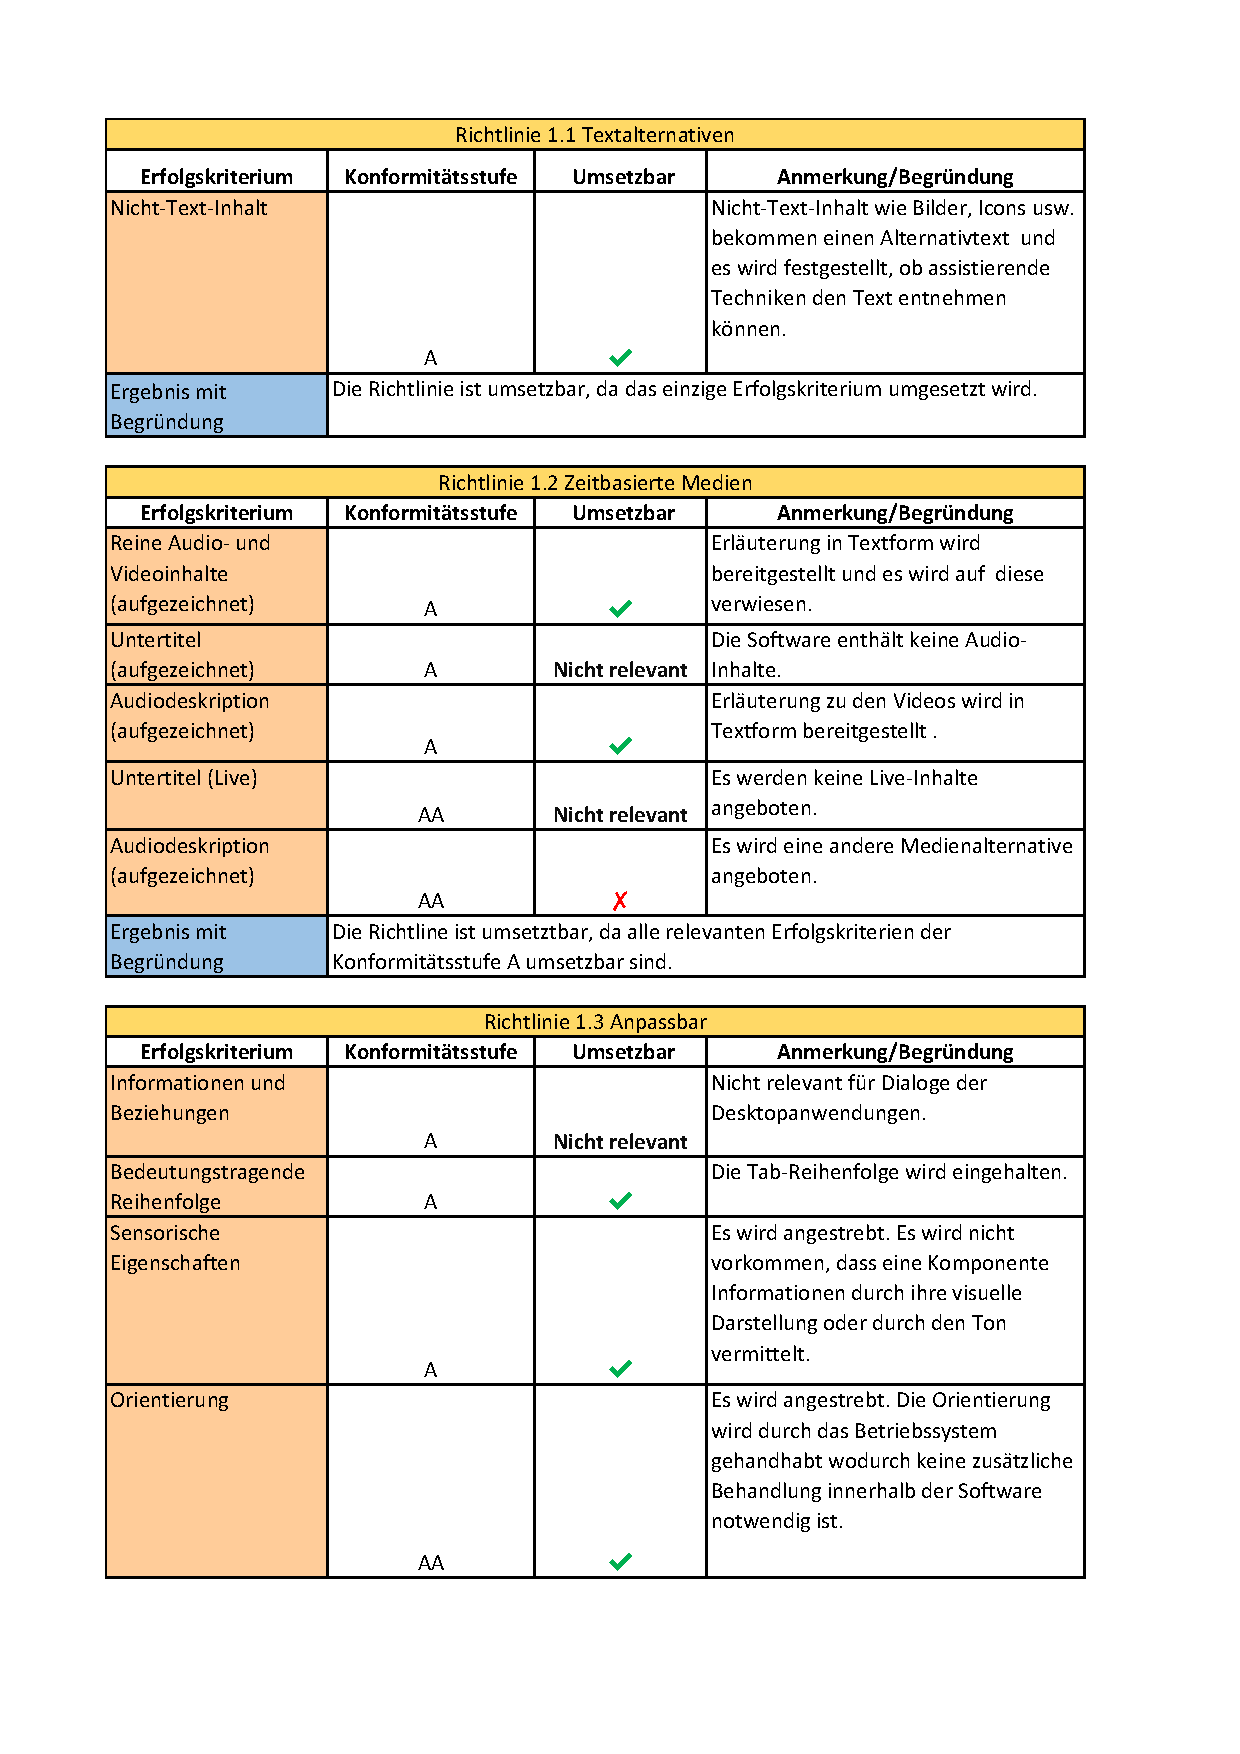
\includepdf[pages=-, scale=0.9, pagecommand={}]{Bewertung der Richtlinien}

\subsubsection{Barrierefreiheit im Software-Entwicklungsprozess}
Beachten die Entwickler die Umsetzung der digitalen Barrierefreiheit von Anfang an nicht, da der Kunde sie im Lastenheft gar nicht verlangt, dann wird eine Umarbeitung der Software sehr aufwendig sein, falls der Kunde sie später doch wünscht.\footnote{Standards für barrierefreie Software \cite{DEVINSIDER}}"`Es empfiehlt sich, bei jeder neuen Entwicklung oder Implementierung, Barrierefreiheit von Anfang an mit zu denken. Zahlreiche Erfahrungen haben gezeigt, dass die Nachrüstung oder Nachbesserung in der Regel deutlich kostenintensiver wird, als die direkte Berücksichtigung."'\footnote{Vgl. Accessibility über Desktopanwendungen hinaus–Barrierefreiheit S. 508 \cite{buhler2017accessibility}}
 
Außerdem ist der Aufwand für das Entwickeln barrierefreier Software von Anfang an geringer als viele Entwickler glauben, da alle  derzeitigen modernen Betriebssysteme globale Funktionen zur Barrierefreiheit anbieten, die der Softwareentwickler dementsprechend nutzen kann, so wie beispielsweise die Bildschirmtastatur, die kontrastreiche Darstellung, die Bildschirmlupe und das Vorlesen von Elementen usw..\footnote{Standards für barrierefreie Software \cite{DEVINSIDER}}

\subsection{Soll-Zustand der Desktopanwendungen}
\label{subsec: Soll-Zustand der Desktopanwendungen}

\comingSoon{+ Die umsetzbare Kriterien werden aufgelistet.\\+ Die Umsetzung erfolgt zu einem späteren Zeitpunkt und nicht in dieser Arbeit.\\+ 4--5 Beispiele für Techniken -> Franz-Josef\\+ Tests werden möglicherweise in einer Folgearbeit betrachtet.}
